\chapter{Introduction}\label{sec:introduction}

\section{The IDSC Cubli}\label{sec:cubli}

\begin{figure}[ht]
   \centering
   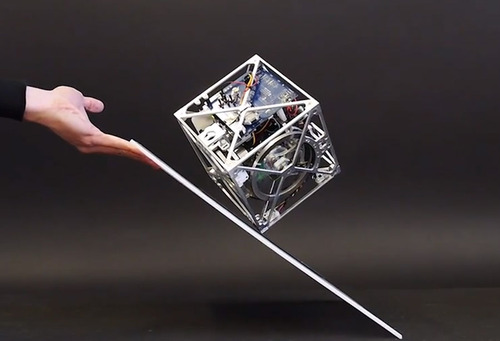
\includegraphics[width=0.75\textwidth]{img/Cubli.jpg}
   \caption{The IDSC Cubli balancing on a slanted surface.}
   \label{img:Cubli}
\end{figure}

The Cubli is a robotic cube developed at the IDSC lab in ETH Zurich, with the ability to balance on its edges and corners by using internal reaction wheels. Of relatively small size, that is dimensions of 15 x 15 x 15 cm, the robot is a proof-of-concept made possible through innovative design and engineering.\\

On top of its ability to balance, Cubli is also able to jump through well-timed braking of the reaction wheels. It can thus jump from a face to an edge, a corner, or from a face directly to the corner. It is also able to spin, and stop spinning when balancing on a corner.

\begin{figure}[ht]
   \centering
   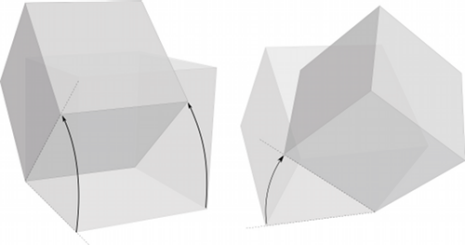
\includegraphics[width=0.75\textwidth]{img/Jumps.png}
   \caption{Illustration of Cubli's jumping abilities.}
   \label{img:Jumps}
\end{figure}

\subsection{Current Interface}

Actions can be executed by pressing buttons visible on one of cubli's faces ( \textit{See Figure \ref{img:Buttons}} ). For example, pressing the Mode button once while holding cubli on its edge at a stable angle will cause it to start balancing. Or, when cubli is on its face, press the mode button once and it jumps up to its edge.\\

\begin{figure}[ht]
   \centering
   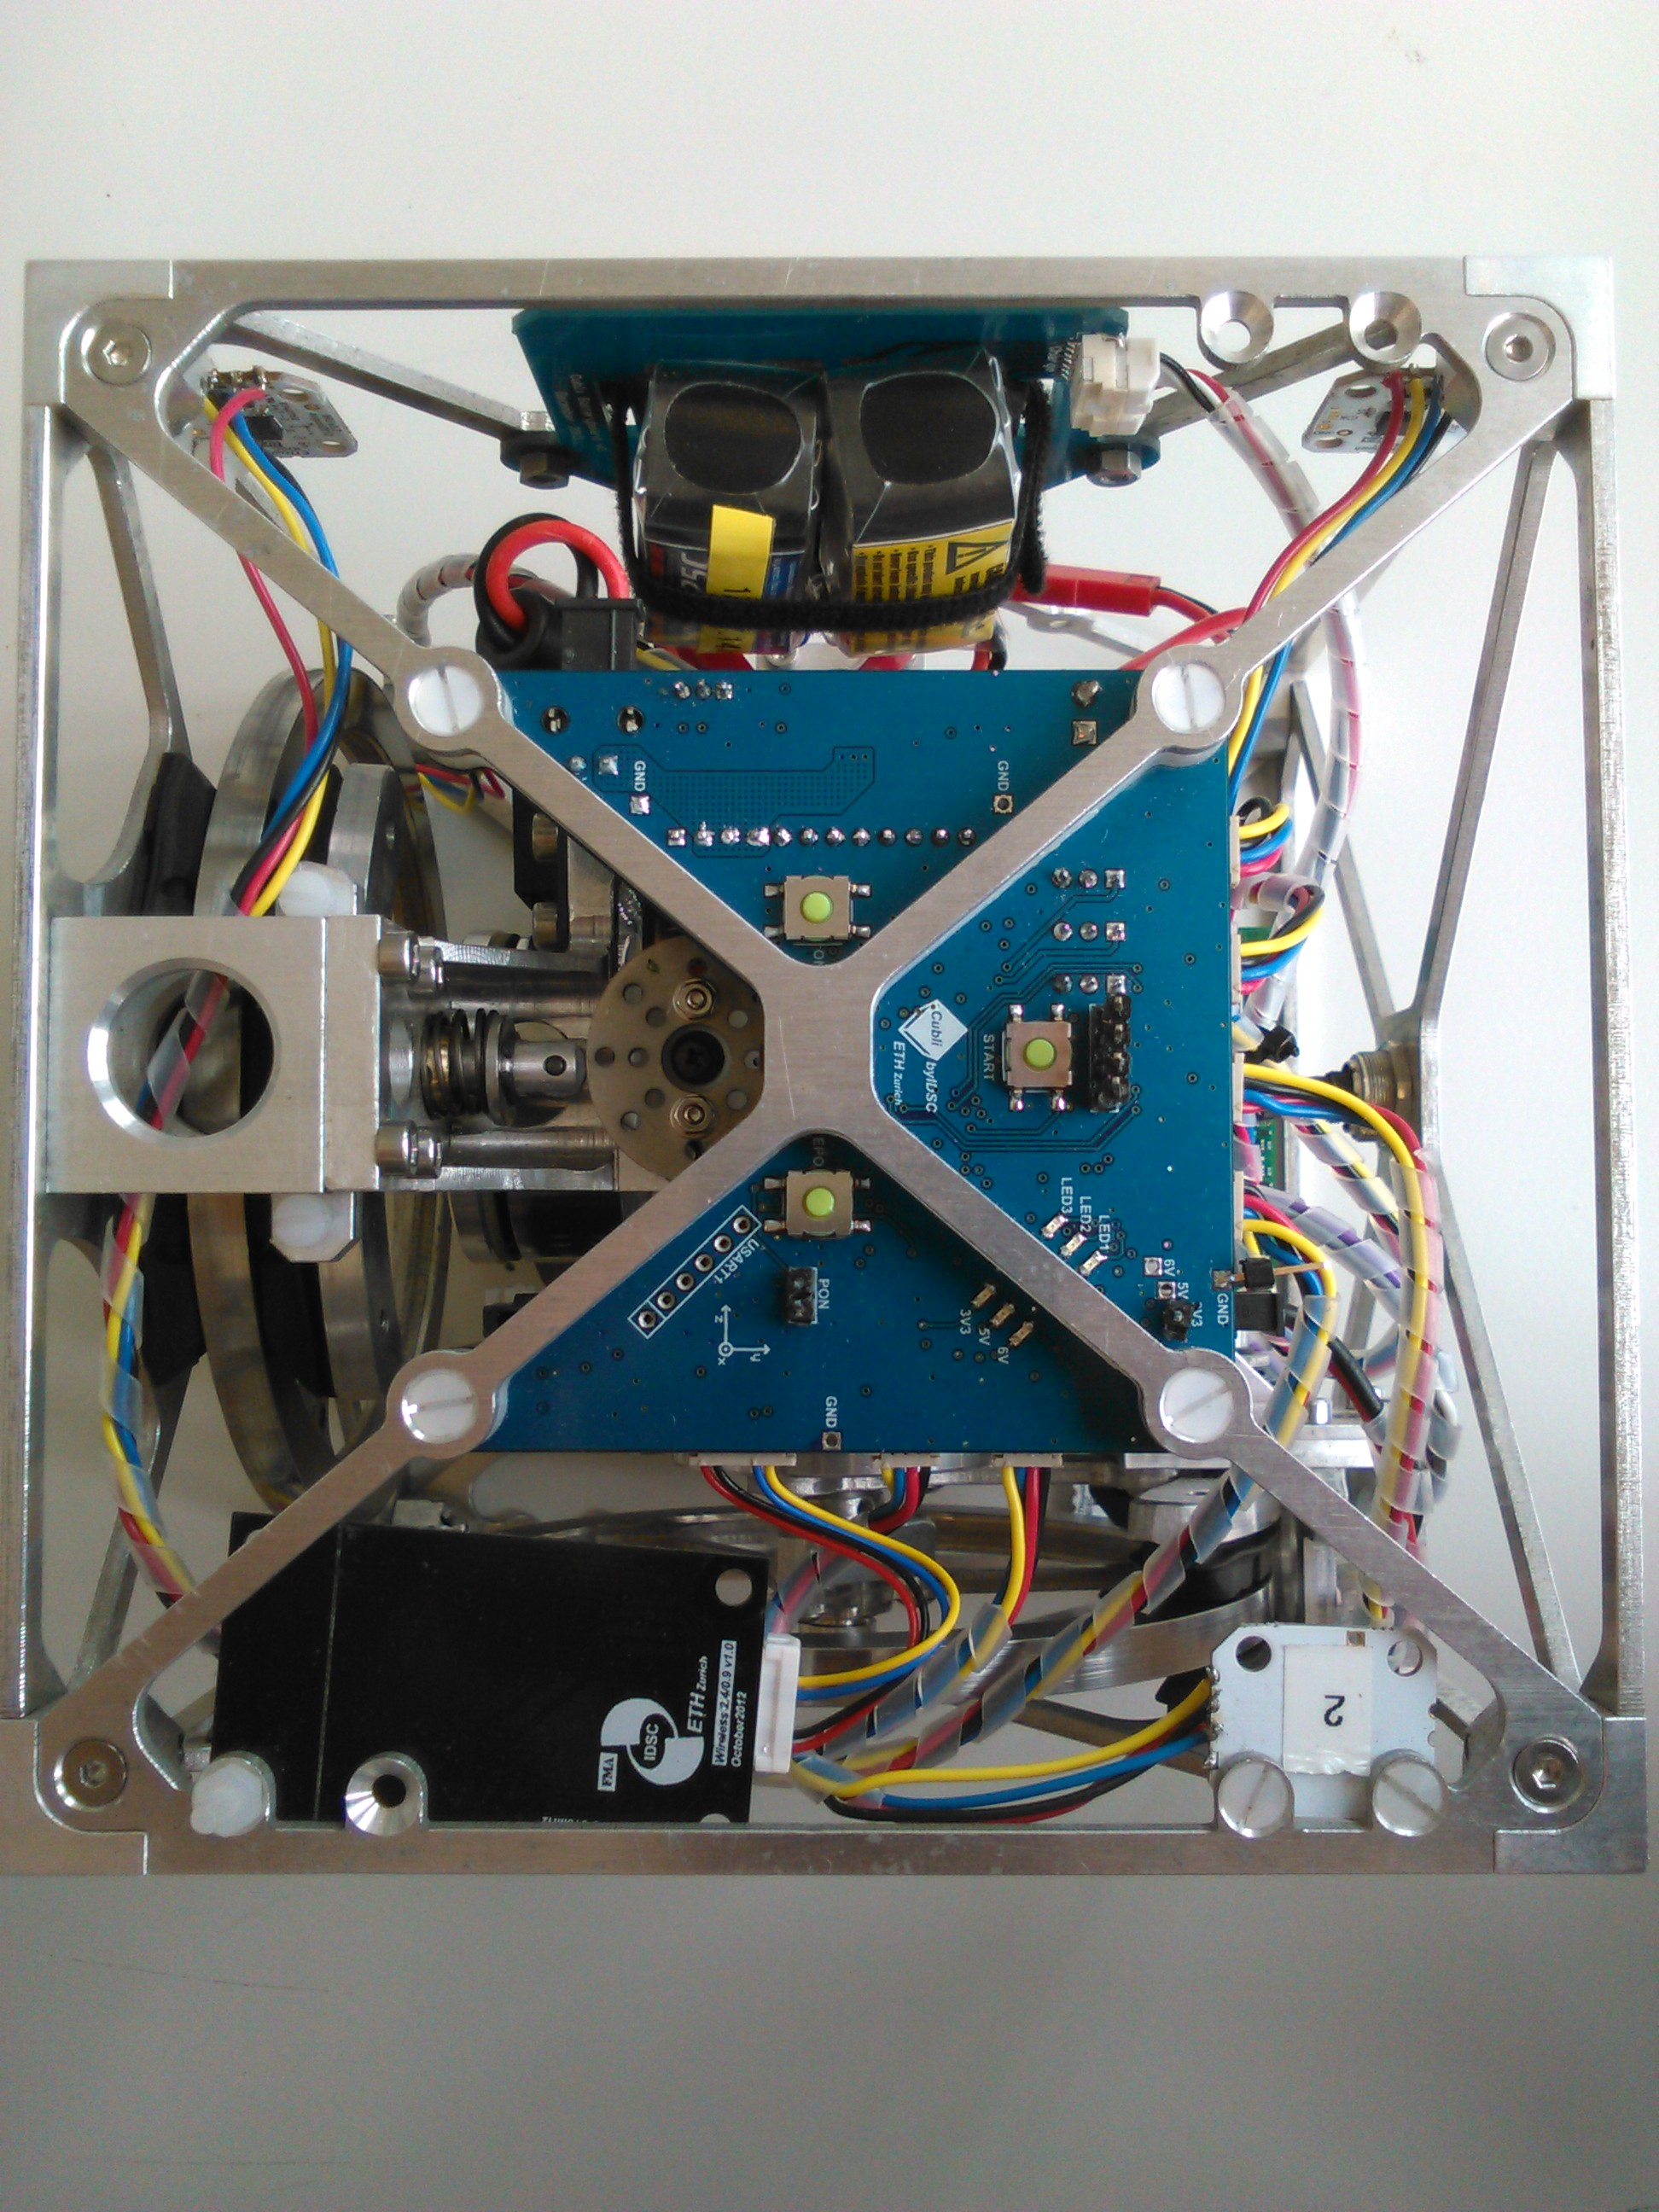
\includegraphics[width=0.75\textwidth]{img/Buttons.jpg}
   \caption{The three buttons on Cubli's controller, used to interact with cubli.}
   \label{img:Buttons}
\end{figure}




